\documentclass[11pt,a4paper]{article}
\usepackage[margin=2.5cm]{geometry}
\usepackage[utf8]{inputenc}
\usepackage[T1]{fontenc}
\usepackage{hyperref}
\renewcommand{\familydefault}{\sfdefault}
\usepackage{helvet}
\pagestyle{empty}
%\usepackage[kerning=true]{microtype}
\usepackage{parskip}
\usepackage{sansmath}
\usepackage[font={small, bf}]{caption}
\usepackage[font={small}]{subcaption}
\usepackage{graphicx}
\usepackage{multicol}
\setlength{\abovecaptionskip}{0pt}
\setlength{\floatsep}{10pt}
\setlength{\textfloatsep}{0pt}
\setlength{\intextsep}{0pt}
\setlength{\belowcaptionskip}{0pt}
\setlength{\parindent}{3ex}
\setlength{\parskip}{0pt}
% Feel free to use additional packages for glosses, figures, whatnot.

% The next bit is for reserving sufficient space for authors,
% affiliations, and e-mail address.  No need to change for initial
% anonymous version.  For the final version, replace the
% \toggletrue{anonymous} with \togglefalse{anonymous} to de-anonymize.
\usepackage{etoolbox}
\newtoggle{anonymous}
\toggletrue{anonymous}
\usepackage{ulem}
\renewcommand{\title}[1]{\textbf{#1}\\}
\newcommand{\authors}[1]{\iftoggle{anonymous}{\phantom{#1}}{#1}\\}
\newcommand{\email}[1]{\iftoggle{anonymous}{\phantom{#1}}{#1}}

\begin{document}



\noindent\title{Context matters: History and informativity affect understanding of opaque references}
\authors{Veronica Boyce (vboyce@stanford.edu), Ben Prystawski, Alvin Tan, Michael C. Frank \\Stanford University}
\newline

\noindent\textbf{Background:} Word predictability (often measured as surprisal) is a predictor of language processing times, but how rapidly do comprehenders adapt to changing contexts that may license expressions that are globally uncommon? Does the use of an unfamiliar shorthand become unsurprising with repeated exposure (based on very local context), or does it stay surprising based on overall unexpectedness? 

 We use transcripts from iterated reference games as a way to create this globally unfamiliar, locally predictable structure. In Boyce et al. 2024\textsuperscript{1}, groups of people played an iterated reference game where a speaker described a target image so that listeners could pick out that target image from a set of 12 images. Over repeated trials, all images were described 6 times. Descriptions from later rounds were shorter and often used opaque descriptions distilled from successful earlier descriptions. Descriptions were in English. 

\smallskip

\noindent \textbf{Methods:} For the present experiment, we selected 10 games with above average accuracy, and above average reduction to in-group nicknames, to test how well outsiders could understand the shorthand descriptions and examine their reading time profile. We recruited 198 English-speaking participants who each read trial transcripts and guessed the intended target. Participants first read the transcript by uncovering it word by word in a modified self-paced reading paradigm, and then selected a target image (Figure 1). In the \textbf{yoked} condition, a participant saw all the trials from one game in the order they occurred (72 trials, 6 descriptions of each of 12 targets). In the \textbf{shuffled} condition, a participant saw all the trials from one game in a randomized order.

\smallskip

\noindent \textbf{Results:} Participants had an average target selection accuracy of 80\% in the yoked condition, and 70\% the in shuffled condition (Figure 2, Table 1).

\indent What predicts word-by-word reading times in this task? In addition to word length and (log) frequency, we considered 3 measures of a word's informativity: \textbf{1)} surprisal from a base large language model (LLM, LLama 3.1 8B)\textsuperscript{2}, \textbf{2)} surprisal from a vision language model (VLM, Llama 3.2 11B)\textsuperscript{2}, conditioned on grid of 12 possible targets, and \textbf{3)} the word-wise change (operationalized as KL divergence) in predicted target distribution from a joint image and text model (CLIP)\textsuperscript{3} with a finetuned classifier head (Figure 3). This last measure represents the task-relevant information content of a word based on how much it shifts the model's distribution over possible targets. We residualized the measures of informativity and normalized all word-level predictors, and then modeled RTs as a function of these predictors for the current and 3 prior words, in addition to condition-level predictors (Figure 4).

\indent Shorter and more frequent words were faster to read, as expected. Unexpectedly, current word LLM surprisal was not predictive, and both VLM surprisal and KL divergence were predictive of shorter reading times, in contrast to the typical positive relationship between surprisal and RTs. LLM surprisal, VLM surprisal, and KL all measure different sources of information with increasing task-specificity, and may have different impulse response functions, leading to different patterns of lag. 

\smallskip 

\noindent\textbf{Discussion:} Language is comprehended in many contexts, in pursuit of many different goals. Here, we examined reading times from participants trying to identify the targets of referential expressions produced in a previous experiment. Judging by their accuracies, participants were able to adapt to the unfamiliar shorthand, especially when they saw the interaction history in order. The RT paradigm used is noisy and prone to spillover effects, but RTs were correlated with word-level predictors such as word length, word frequency, and measures of information.  Further work could refine the measures using more sensitive techniques such as eye-tracking, analyses that better account for time course, and measures of information that take prior informativity into account.


\newpage

\begin{center}\textbf{}\end{center}
%\begin{minipage}{.4\textwidth}
%	\captionof{figure}{Original game}
%	{	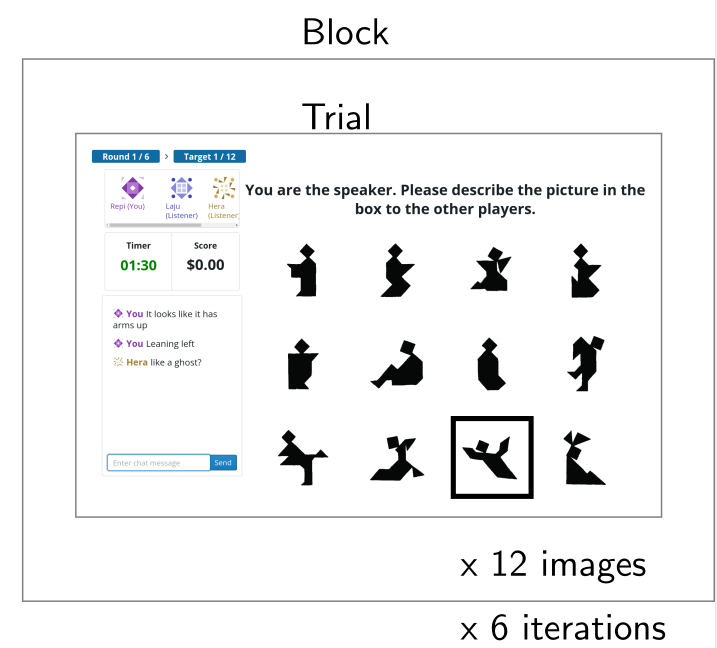
\includegraphics[width=\textwidth]{orig_diagram.png}} 
%	
%	\begin{small}
%	In [articipants played a reference game in real time with other participants using a chat box.
%	
%\end{small}
%	
%\end{minipage}
%~~~
%\begin{minipage}{.55\textwidth}
%	\captionof{figure}{Current experiment}
%	{	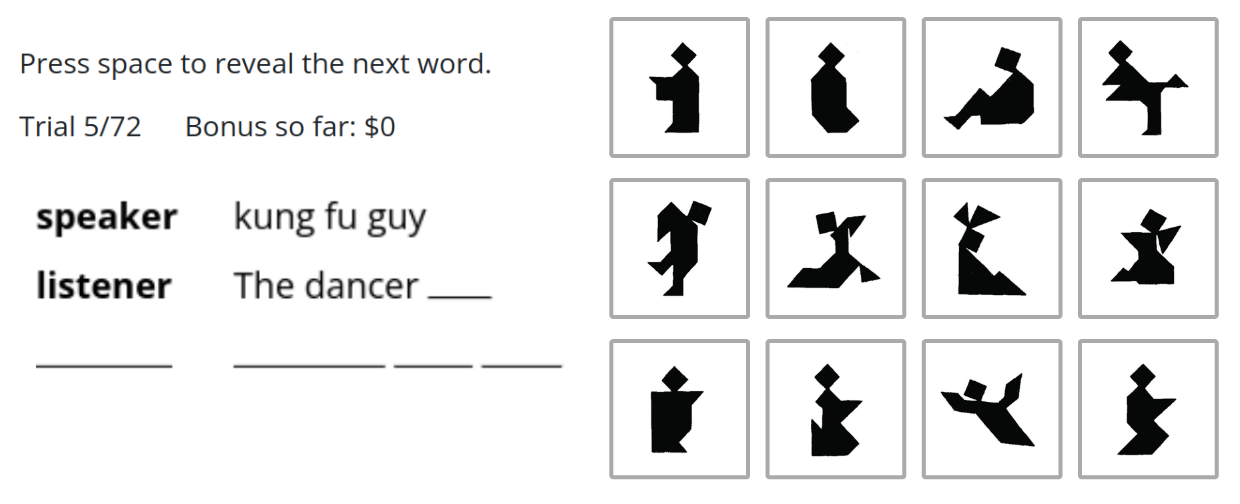
\includegraphics[width=\textwidth]{matcher_diagram.png}} 
%	\begin{small}
%		In the current experiment, we sampled the game transcripts from 10 games from Boyce et al. 2024\textsuperscript{1}. We recruited new participants to each see the transcripts from one game, either with the trials in the same order (yoked) or a random order (shuffled).  New participants revealed the dialogue from a trial word-by-word and then selected what image they think was being described. 
%		
%	\end{small}	
%\end{minipage}


\begin{minipage}{.55\textwidth}
		\captionof{figure}{Experimental set-up}
	{	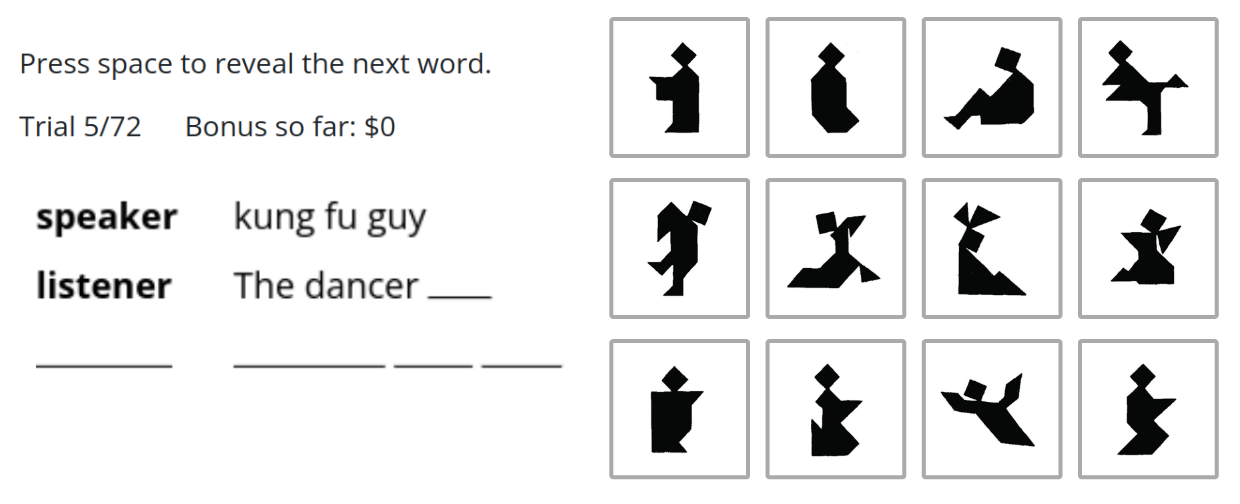
\includegraphics[width=\textwidth]{matcher_diagram.png}} 
	\end{minipage}
~~~
\begin{minipage}{.4\textwidth}

\begin{small}
	In the current experiment, we sampled the game transcripts from 10 games from Boyce et al. 2024\textsuperscript{1}. We recruited new participants to each see the transcripts from one game, either with the trials in the same order (yoked) or a random order (shuffled) for 72 trials.  Participants revealed each trial transcript word by word and then selected the image they thought was being described. 
	
\end{small}	
\end{minipage}

\bigskip

\begin{minipage}{.45\textwidth}
	\captionof{figure}{Accuracy}
	{	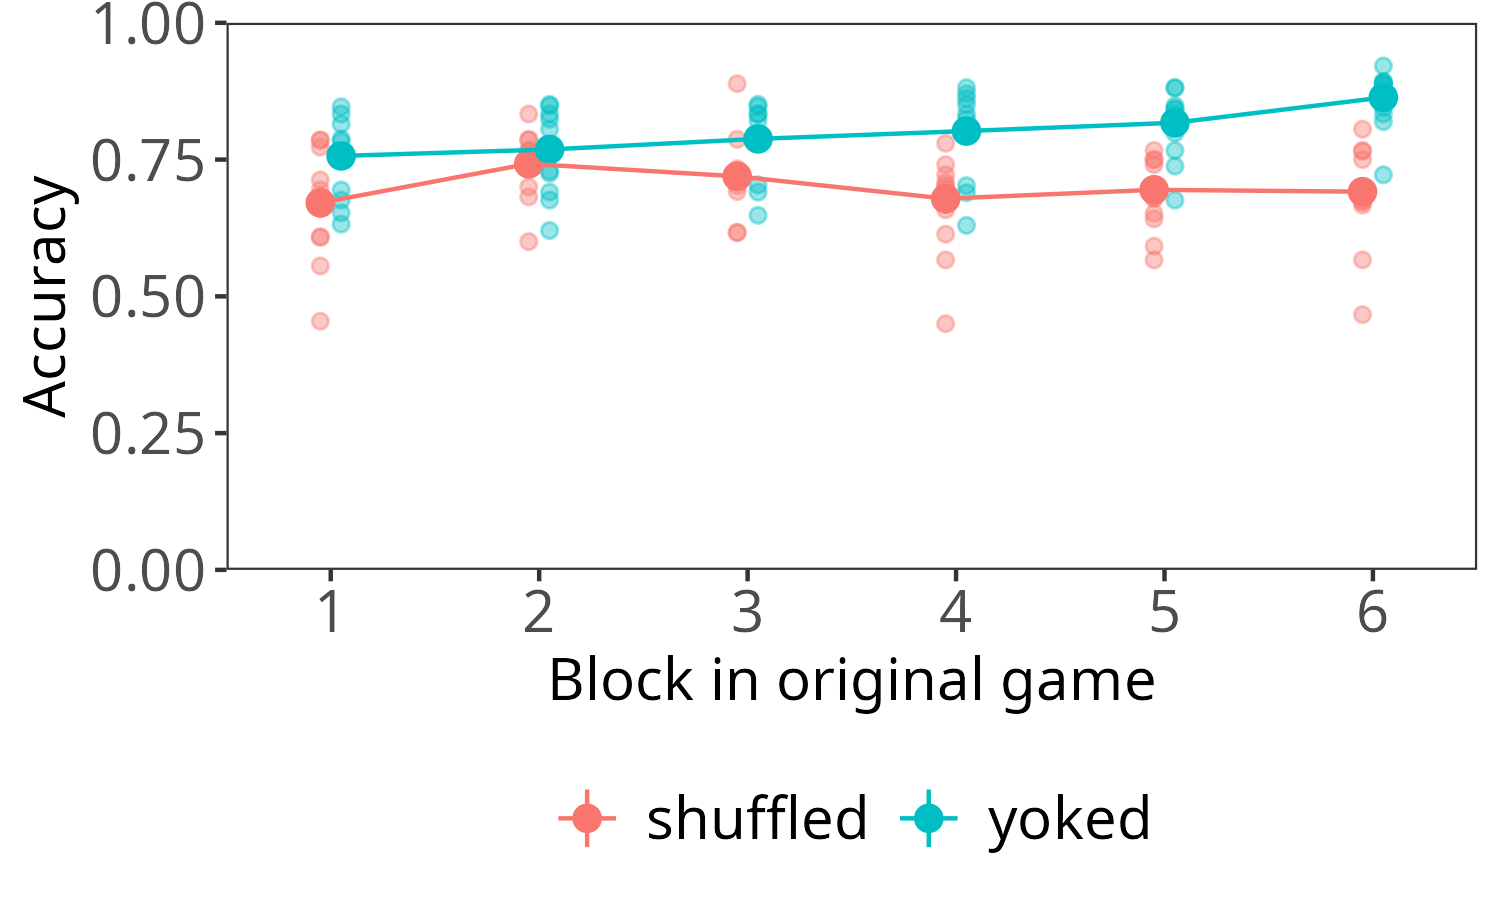
\includegraphics[width=\textwidth]{hsp1.png}} 
	\begin{small}
%
		
	\end{small}
	
\end{minipage}
~~
\begin{minipage}{.5\textwidth}
	\begin{small}
\captionof{table}{Accuracy model}

	\begin{tabular}{|l|l|l|}
		\hline
		Term & Odds Ratio & 95\% CrI \\
		\hline
		Intercept & 1.574 & [.891 -- 2.834] \\
		Original Block & .986 & [.954 -- 1.020] \\ 
		Condition (yoked) & 2.196 & [1.634 -- 3.002] \\
		Block x Condition & .944 & [.889 -- 1.002] \\
		Viewing order & 1.019 & [1.016 -- 1.021] \\
		\hline
	\end{tabular}
	\vspace{2pt}
	
	 Logistic Model: \textit{Accuracy $\sim$  original-block $\times$ condition + order-viewed + (1 | game) + (1 | target) + (1 | participant)  } Coefficients are presented as odds ratios (how much more likely correct responses are).
	 
	 \end{small}
	 	
\end{minipage}

\bigskip



\begin{minipage}{.5\textwidth}
	\captionof{figure}{Informativity Predictors}
	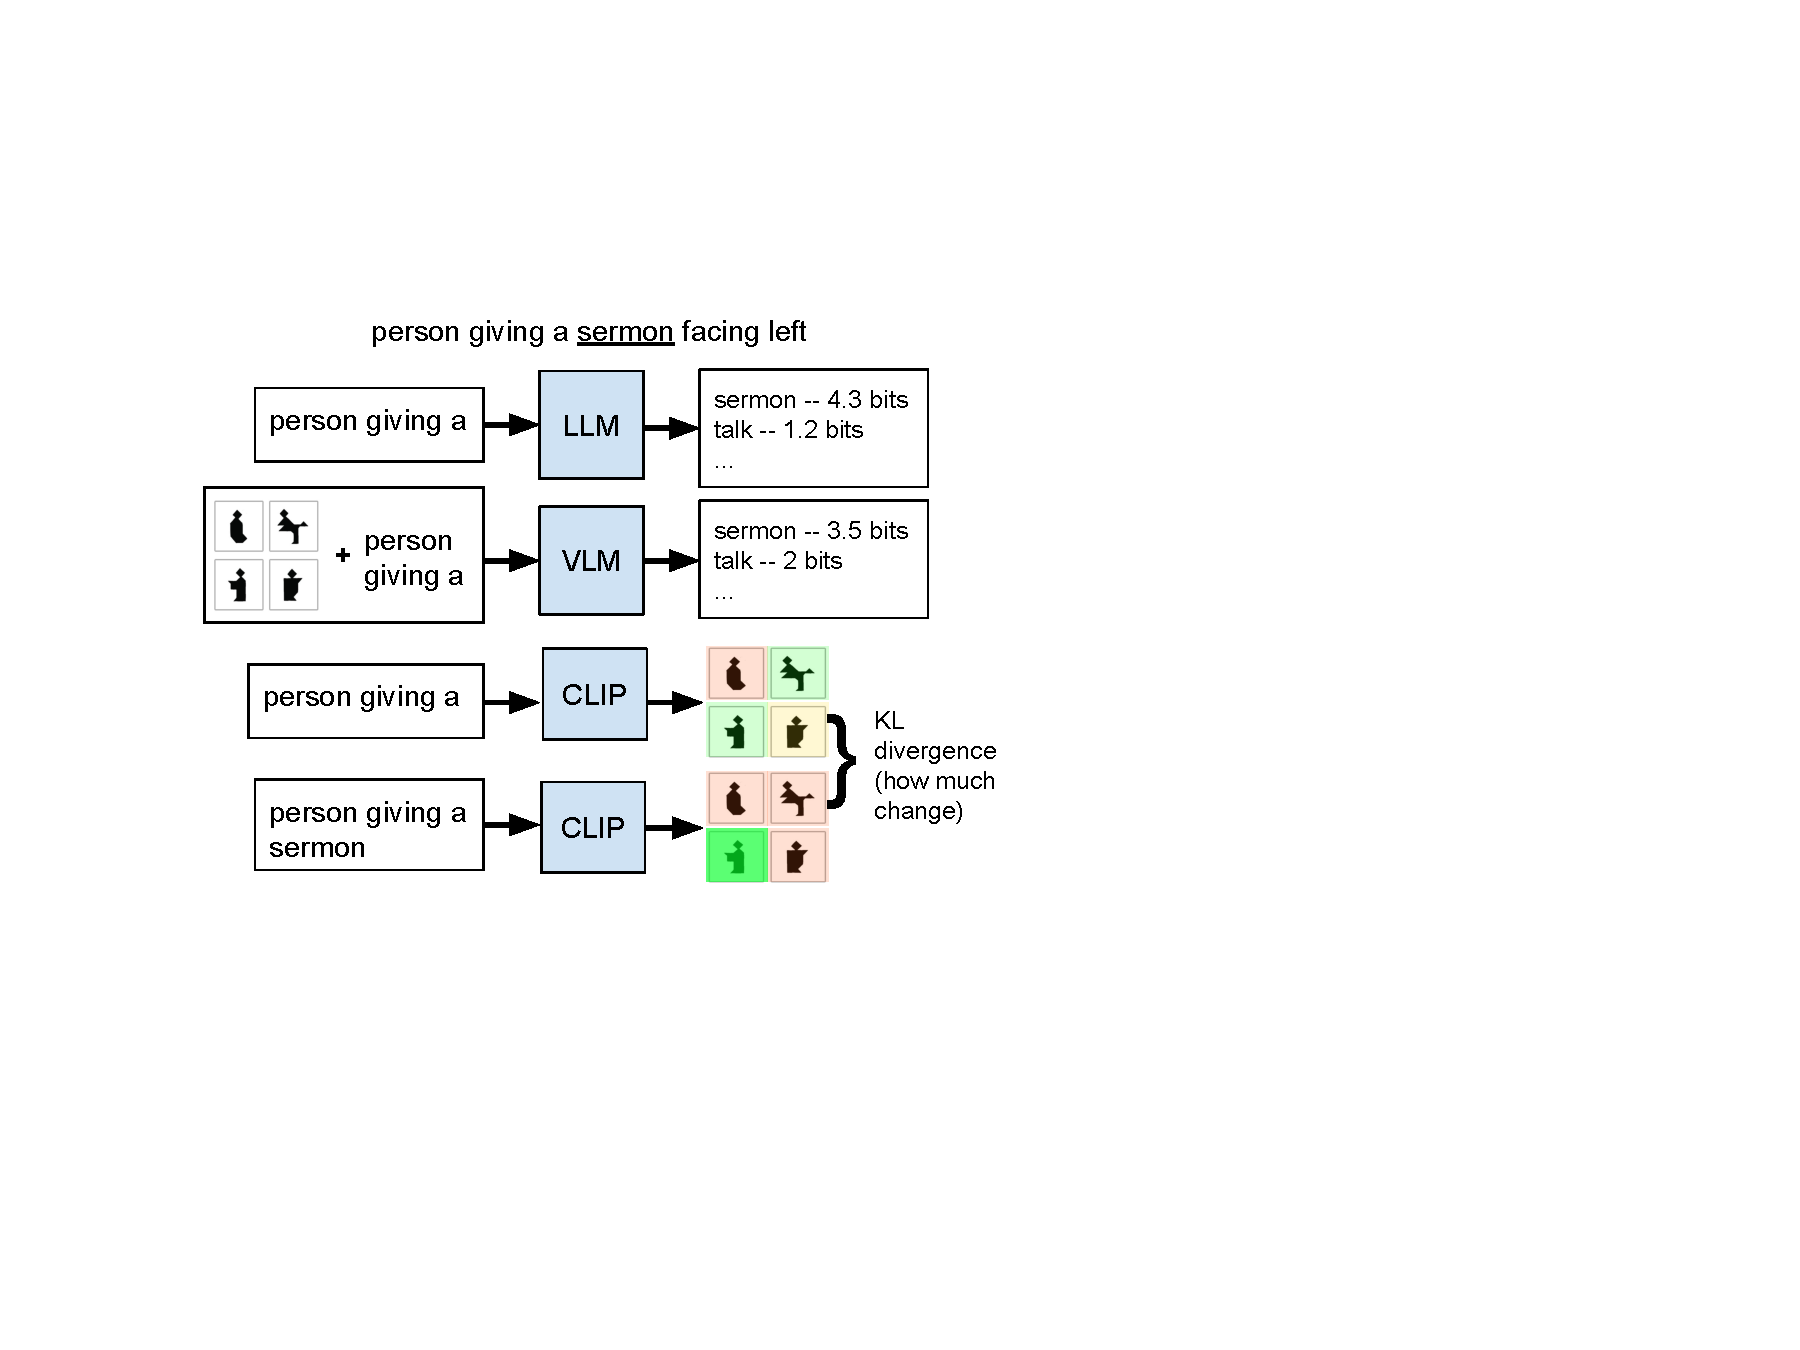
\includegraphics[width=\textwidth, trim = 3.2cm 7.7cm 13.5cm 6cm, clip]{preds.pdf} 

	
\end{minipage}
~~
\begin{minipage}{.45\textwidth}
	\begin{small}
	We considered 3 different sources for the information content of a word, here shown for the word ``sermon''. We used Llama 3.1 8B for the LLM, and Llama 3.2 11B for the VLM. The CLIP model used a finetuned classifer head trained on the Boyce et al. 2024\textsuperscript{1} corpora.
	
	\smallskip
	
LLM surprisal was residualized off of word length and word frequency. VLM surprisal and KL divergence were residualized off of word length, word frequency, and LLM surprisal. All word-level predictors were normalized. 
	
\end{small}
	
\end{minipage}

\bigskip

\begin{minipage}{.5\textwidth}
		\captionof{figure}{RT model}
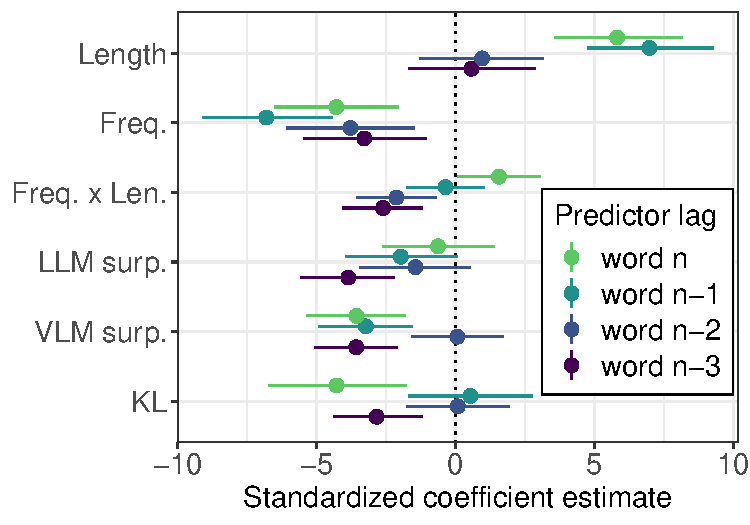
\includegraphics[width=\textwidth]{word_preds.pdf} 
	
\end{minipage}
~~
\begin{minipage}{.45\textwidth}
	\begin{small}

		
		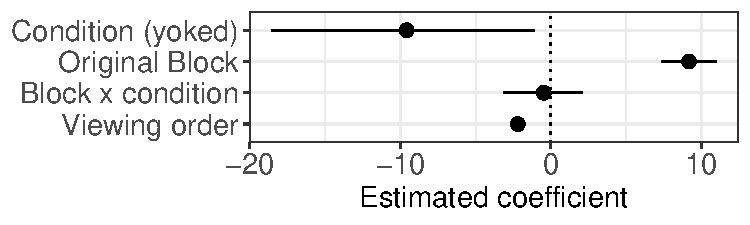
\includegraphics[width=\textwidth]{other_preds.pdf} 
		
		\vspace{2pt}
		
		Model: \textit{RT $\sim$ [word-length $\times$ frequency + LLM + VLM + KL] +  original-block $\times$ condition + order-viewed + (1 | game) + (1 | target) + (1 | participant)  } Bracketed predictors were included for current word and 3 prior words to account for spillover. 
		
	\end{small}
	
\end{minipage}

	\bigskip

\begin{minipage}{\textwidth}
	\vspace{5pt}
	\begin{small} \textbf{References:}%TODO update
		
1. Boyce, Hawkins, Goodman, Frank. PNAS, 2024. $\bullet$
2. Grattafiori et al., arXiv, 2024. arXiv:2407.21783 $\bullet$
3. Radford et al. arXiv, 2021. arXiv:2103.00020 

\end{small}
\end{minipage}


\end{document}